% Options for packages loaded elsewhere
\PassOptionsToPackage{unicode}{hyperref}
\PassOptionsToPackage{hyphens}{url}
%
\documentclass[
]{article}
\usepackage{amsmath,amssymb}
\usepackage{lmodern}
\usepackage{iftex}
\ifPDFTeX
  \usepackage[T1]{fontenc}
  \usepackage[utf8]{inputenc}
  \usepackage{textcomp} % provide euro and other symbols
\else % if luatex or xetex
  \usepackage{unicode-math}
  \defaultfontfeatures{Scale=MatchLowercase}
  \defaultfontfeatures[\rmfamily]{Ligatures=TeX,Scale=1}
\fi
% Use upquote if available, for straight quotes in verbatim environments
\IfFileExists{upquote.sty}{\usepackage{upquote}}{}
\IfFileExists{microtype.sty}{% use microtype if available
  \usepackage[]{microtype}
  \UseMicrotypeSet[protrusion]{basicmath} % disable protrusion for tt fonts
}{}
\makeatletter
\@ifundefined{KOMAClassName}{% if non-KOMA class
  \IfFileExists{parskip.sty}{%
    \usepackage{parskip}
  }{% else
    \setlength{\parindent}{0pt}
    \setlength{\parskip}{6pt plus 2pt minus 1pt}}
}{% if KOMA class
  \KOMAoptions{parskip=half}}
\makeatother
\usepackage{xcolor}
\usepackage[margin=1in]{geometry}
\usepackage{color}
\usepackage{fancyvrb}
\newcommand{\VerbBar}{|}
\newcommand{\VERB}{\Verb[commandchars=\\\{\}]}
\DefineVerbatimEnvironment{Highlighting}{Verbatim}{commandchars=\\\{\}}
% Add ',fontsize=\small' for more characters per line
\usepackage{framed}
\definecolor{shadecolor}{RGB}{248,248,248}
\newenvironment{Shaded}{\begin{snugshade}}{\end{snugshade}}
\newcommand{\AlertTok}[1]{\textcolor[rgb]{0.94,0.16,0.16}{#1}}
\newcommand{\AnnotationTok}[1]{\textcolor[rgb]{0.56,0.35,0.01}{\textbf{\textit{#1}}}}
\newcommand{\AttributeTok}[1]{\textcolor[rgb]{0.77,0.63,0.00}{#1}}
\newcommand{\BaseNTok}[1]{\textcolor[rgb]{0.00,0.00,0.81}{#1}}
\newcommand{\BuiltInTok}[1]{#1}
\newcommand{\CharTok}[1]{\textcolor[rgb]{0.31,0.60,0.02}{#1}}
\newcommand{\CommentTok}[1]{\textcolor[rgb]{0.56,0.35,0.01}{\textit{#1}}}
\newcommand{\CommentVarTok}[1]{\textcolor[rgb]{0.56,0.35,0.01}{\textbf{\textit{#1}}}}
\newcommand{\ConstantTok}[1]{\textcolor[rgb]{0.00,0.00,0.00}{#1}}
\newcommand{\ControlFlowTok}[1]{\textcolor[rgb]{0.13,0.29,0.53}{\textbf{#1}}}
\newcommand{\DataTypeTok}[1]{\textcolor[rgb]{0.13,0.29,0.53}{#1}}
\newcommand{\DecValTok}[1]{\textcolor[rgb]{0.00,0.00,0.81}{#1}}
\newcommand{\DocumentationTok}[1]{\textcolor[rgb]{0.56,0.35,0.01}{\textbf{\textit{#1}}}}
\newcommand{\ErrorTok}[1]{\textcolor[rgb]{0.64,0.00,0.00}{\textbf{#1}}}
\newcommand{\ExtensionTok}[1]{#1}
\newcommand{\FloatTok}[1]{\textcolor[rgb]{0.00,0.00,0.81}{#1}}
\newcommand{\FunctionTok}[1]{\textcolor[rgb]{0.00,0.00,0.00}{#1}}
\newcommand{\ImportTok}[1]{#1}
\newcommand{\InformationTok}[1]{\textcolor[rgb]{0.56,0.35,0.01}{\textbf{\textit{#1}}}}
\newcommand{\KeywordTok}[1]{\textcolor[rgb]{0.13,0.29,0.53}{\textbf{#1}}}
\newcommand{\NormalTok}[1]{#1}
\newcommand{\OperatorTok}[1]{\textcolor[rgb]{0.81,0.36,0.00}{\textbf{#1}}}
\newcommand{\OtherTok}[1]{\textcolor[rgb]{0.56,0.35,0.01}{#1}}
\newcommand{\PreprocessorTok}[1]{\textcolor[rgb]{0.56,0.35,0.01}{\textit{#1}}}
\newcommand{\RegionMarkerTok}[1]{#1}
\newcommand{\SpecialCharTok}[1]{\textcolor[rgb]{0.00,0.00,0.00}{#1}}
\newcommand{\SpecialStringTok}[1]{\textcolor[rgb]{0.31,0.60,0.02}{#1}}
\newcommand{\StringTok}[1]{\textcolor[rgb]{0.31,0.60,0.02}{#1}}
\newcommand{\VariableTok}[1]{\textcolor[rgb]{0.00,0.00,0.00}{#1}}
\newcommand{\VerbatimStringTok}[1]{\textcolor[rgb]{0.31,0.60,0.02}{#1}}
\newcommand{\WarningTok}[1]{\textcolor[rgb]{0.56,0.35,0.01}{\textbf{\textit{#1}}}}
\usepackage{graphicx}
\makeatletter
\def\maxwidth{\ifdim\Gin@nat@width>\linewidth\linewidth\else\Gin@nat@width\fi}
\def\maxheight{\ifdim\Gin@nat@height>\textheight\textheight\else\Gin@nat@height\fi}
\makeatother
% Scale images if necessary, so that they will not overflow the page
% margins by default, and it is still possible to overwrite the defaults
% using explicit options in \includegraphics[width, height, ...]{}
\setkeys{Gin}{width=\maxwidth,height=\maxheight,keepaspectratio}
% Set default figure placement to htbp
\makeatletter
\def\fps@figure{htbp}
\makeatother
\setlength{\emergencystretch}{3em} % prevent overfull lines
\providecommand{\tightlist}{%
  \setlength{\itemsep}{0pt}\setlength{\parskip}{0pt}}
\setcounter{secnumdepth}{-\maxdimen} % remove section numbering
\ifLuaTeX
  \usepackage{selnolig}  % disable illegal ligatures
\fi
\IfFileExists{bookmark.sty}{\usepackage{bookmark}}{\usepackage{hyperref}}
\IfFileExists{xurl.sty}{\usepackage{xurl}}{} % add URL line breaks if available
\urlstyle{same} % disable monospaced font for URLs
\hypersetup{
  pdftitle={computer-related-offense.R},
  pdfauthor={jasmeen},
  hidelinks,
  pdfcreator={LaTeX via pandoc}}

\title{computer-related-offense.R}
\author{jasmeen}
\date{2023-03-26}

\begin{document}
\maketitle

\begin{Shaded}
\begin{Highlighting}[]
\FunctionTok{library}\NormalTok{(readxl)}
\NormalTok{data}\OtherTok{=}\FunctionTok{read\_excel}\NormalTok{(}\StringTok{"computer related offense.xlsx"}\NormalTok{)}
\NormalTok{data}
\end{Highlighting}
\end{Shaded}

\begin{verbatim}
## # A tibble: 8 x 2
##    year CasesReported
##   <dbl>         <dbl>
## 1  2014          5548
## 2  2015          6567
## 3  2016          6818
## 4  2017         10108
## 5  2018         14141
## 6  2019         23612
## 7  2020         21926
## 8  2021         19915
\end{verbatim}

\begin{Shaded}
\begin{Highlighting}[]
\NormalTok{x}\OtherTok{=}\NormalTok{data}\SpecialCharTok{$}\NormalTok{year}
\NormalTok{y}\OtherTok{=}\NormalTok{data}\SpecialCharTok{$}\NormalTok{CasesReported}
\FunctionTok{plot}\NormalTok{(data,}\AttributeTok{pch=}\DecValTok{20}\NormalTok{,}\AttributeTok{col=}\StringTok{"blue4"}\NormalTok{)}
\FunctionTok{lines}\NormalTok{(data)}
\end{Highlighting}
\end{Shaded}

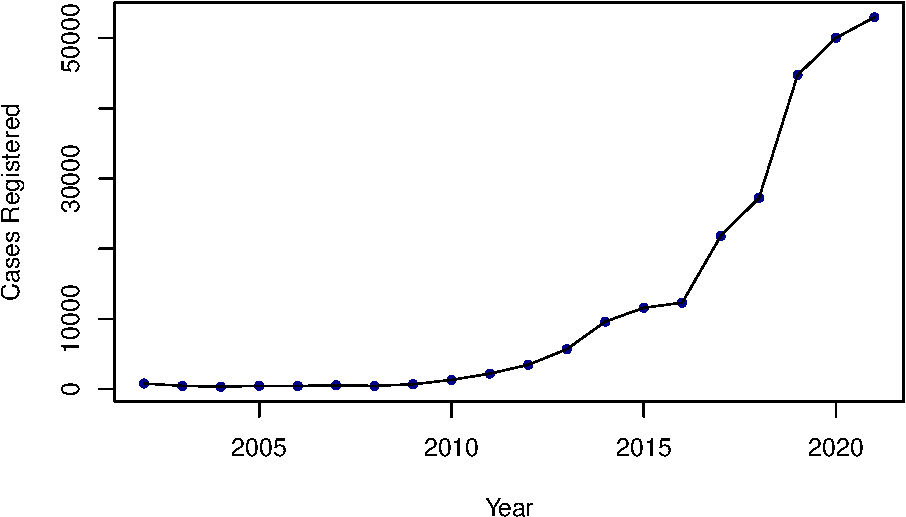
\includegraphics{computer-related-offense_files/figure-latex/unnamed-chunk-1-1.pdf}

\begin{Shaded}
\begin{Highlighting}[]
\NormalTok{model1}\OtherTok{=}\FunctionTok{lm}\NormalTok{(y}\SpecialCharTok{\textasciitilde{}}\NormalTok{x)}
\FunctionTok{summary}\NormalTok{(model1)}
\end{Highlighting}
\end{Shaded}

\begin{verbatim}
## 
## Call:
## lm(formula = y ~ x)
## 
## Residuals:
##     Min      1Q  Median      3Q     Max 
## -3321.8 -2224.4  -466.1  1492.9  5893.7 
## 
## Coefficients:
##               Estimate Std. Error t value Pr(>|t|)   
## (Intercept) -5553255.5  1004317.1  -5.529  0.00147 **
## x               2759.3      497.8   5.543  0.00146 **
## ---
## Signif. codes:  0 '***' 0.001 '**' 0.01 '*' 0.05 '.' 0.1 ' ' 1
## 
## Residual standard error: 3226 on 6 degrees of freedom
## Multiple R-squared:  0.8366, Adjusted R-squared:  0.8094 
## F-statistic: 30.72 on 1 and 6 DF,  p-value: 0.001456
\end{verbatim}

\begin{Shaded}
\begin{Highlighting}[]
\NormalTok{model2}\OtherTok{=}\FunctionTok{lm}\NormalTok{(y}\SpecialCharTok{\textasciitilde{}}\FunctionTok{poly}\NormalTok{(x,}\DecValTok{2}\NormalTok{,}\AttributeTok{raw =} \ConstantTok{TRUE}\NormalTok{))}
\FunctionTok{summary}\NormalTok{(model2)}
\end{Highlighting}
\end{Shaded}

\begin{verbatim}
## 
## Call:
## lm(formula = y ~ poly(x, 2, raw = TRUE))
## 
## Residuals:
##        1        2        3        4        5        6        7        8 
##  1867.79   -79.66 -2726.05 -2264.39  -990.66  5790.13  1482.97 -3080.13 
## 
## Coefficients:
##                           Estimate Std. Error t value Pr(>|t|)
## (Intercept)             -1.461e+08  1.108e+09  -0.132    0.900
## poly(x, 2, raw = TRUE)1  1.421e+05  1.098e+06   0.129    0.902
## poly(x, 2, raw = TRUE)2 -3.453e+01  2.722e+02  -0.127    0.904
## 
## Residual standard error: 3528 on 5 degrees of freedom
## Multiple R-squared:  0.8371, Adjusted R-squared:  0.772 
## F-statistic: 12.85 on 2 and 5 DF,  p-value: 0.0107
\end{verbatim}

\begin{Shaded}
\begin{Highlighting}[]
\NormalTok{model3 }\OtherTok{=} \FunctionTok{lm}\NormalTok{(}\FunctionTok{log}\NormalTok{(y) }\SpecialCharTok{\textasciitilde{}}\NormalTok{ x)}
\FunctionTok{summary}\NormalTok{(model3)}
\end{Highlighting}
\end{Shaded}

\begin{verbatim}
## 
## Call:
## lm(formula = log(y) ~ x)
## 
## Residuals:
##      Min       1Q   Median       3Q      Max 
## -0.26652 -0.07994  0.01283  0.05997  0.35702 
## 
## Coefficients:
##               Estimate Std. Error t value Pr(>|t|)    
## (Intercept) -447.84694   63.83852  -7.015 0.000418 ***
## x              0.22663    0.03164   7.162 0.000374 ***
## ---
## Signif. codes:  0 '***' 0.001 '**' 0.01 '*' 0.05 '.' 0.1 ' ' 1
## 
## Residual standard error: 0.2051 on 6 degrees of freedom
## Multiple R-squared:  0.8953, Adjusted R-squared:  0.8778 
## F-statistic:  51.3 on 1 and 6 DF,  p-value: 0.0003739
\end{verbatim}

\begin{Shaded}
\begin{Highlighting}[]
\NormalTok{x\_axis}\OtherTok{=}\DecValTok{2014}\SpecialCharTok{:}\DecValTok{2021}
\FunctionTok{data.frame}\NormalTok{(}\AttributeTok{year=}\NormalTok{data}\SpecialCharTok{$}\NormalTok{year,}\AttributeTok{actual =}\NormalTok{ data}\SpecialCharTok{$}\NormalTok{CasesReported,}\AttributeTok{linear=}\FunctionTok{predict}\NormalTok{(model1,}\FunctionTok{data.frame}\NormalTok{(}\AttributeTok{x=}\NormalTok{x\_axis)),}\AttributeTok{quad =} \FunctionTok{predict}\NormalTok{(model2,}\FunctionTok{data.frame}\NormalTok{(}\AttributeTok{x=}\NormalTok{x\_axis)),}\AttributeTok{loge =} \FunctionTok{exp}\NormalTok{(}\FunctionTok{predict}\NormalTok{(model3,}\FunctionTok{data.frame}\NormalTok{(}\AttributeTok{x=}\NormalTok{x\_axis))) )}
\end{Highlighting}
\end{Shaded}

\begin{verbatim}
##   year actual    linear      quad      loge
## 1 2014   5548  3921.917  3680.208  5320.686
## 2 2015   6567  6681.190  6646.661  6674.065
## 3 2016   6818  9440.464  9544.054  8371.690
## 4 2017  10108 12199.738 12372.387 10501.127
## 5 2018  14141 14959.012 15131.661 13172.211
## 6 2019  23612 17718.286 17821.875 16522.715
## 7 2020  21926 20477.560 20443.030 20725.460
## 8 2021  19915 23236.833 22995.125 25997.221
\end{verbatim}

\begin{Shaded}
\begin{Highlighting}[]
\FunctionTok{plot}\NormalTok{(data,}\AttributeTok{pch=}\DecValTok{20}\NormalTok{,}\AttributeTok{col=}\StringTok{"blue4"}\NormalTok{)}
\NormalTok{m3}\OtherTok{=}\ControlFlowTok{function}\NormalTok{(x)\{}
  \FunctionTok{exp}\NormalTok{(}\SpecialCharTok{{-}}\FloatTok{524.60367+0.26470}\SpecialCharTok{*}\NormalTok{x)}
\NormalTok{\}}
\FunctionTok{curve}\NormalTok{(m3,}\AttributeTok{from =} \DecValTok{2014}\NormalTok{ ,}\AttributeTok{to =} \DecValTok{2021}\NormalTok{,}\AttributeTok{add =} \ConstantTok{TRUE}\NormalTok{ ,}\AttributeTok{lwd =} \FloatTok{1.5}\NormalTok{ , }\AttributeTok{col =} \StringTok{"blue"}\NormalTok{)}
\end{Highlighting}
\end{Shaded}

\includegraphics{computer-related-offense_files/figure-latex/unnamed-chunk-1-2.pdf}

\begin{Shaded}
\begin{Highlighting}[]
\DocumentationTok{\#\#calculate percentage increase in x}
\FunctionTok{rm}\NormalTok{(}\AttributeTok{list =} \FunctionTok{ls}\NormalTok{())}
\NormalTok{y1}\OtherTok{=}\DecValTok{2014}\SpecialCharTok{:}\DecValTok{2021}
\NormalTok{x1}\OtherTok{=}\FunctionTok{c}\NormalTok{(}\DecValTok{5548}\NormalTok{,}\DecValTok{6567}\NormalTok{,}\DecValTok{6818}\NormalTok{,}\DecValTok{10108}\NormalTok{,}\DecValTok{14141}\NormalTok{,}\DecValTok{23612}\NormalTok{,}\DecValTok{21926}\NormalTok{,}\DecValTok{19915}\NormalTok{)}
\NormalTok{df}\OtherTok{=}\FunctionTok{data.frame}\NormalTok{(y1,x1)}
\NormalTok{df}
\end{Highlighting}
\end{Shaded}

\begin{verbatim}
##     y1    x1
## 1 2014  5548
## 2 2015  6567
## 3 2016  6818
## 4 2017 10108
## 5 2018 14141
## 6 2019 23612
## 7 2020 21926
## 8 2021 19915
\end{verbatim}

\begin{Shaded}
\begin{Highlighting}[]
\NormalTok{pinc}\OtherTok{=}\ControlFlowTok{function}\NormalTok{(x)\{}
\NormalTok{  per\_inc }\OtherTok{=} \FunctionTok{c}\NormalTok{()}
  \ControlFlowTok{for}\NormalTok{(i }\ControlFlowTok{in} \DecValTok{2}\SpecialCharTok{:}\FunctionTok{length}\NormalTok{(x))\{}
\NormalTok{    per\_inc[i] }\OtherTok{=}\NormalTok{ x[i]}\SpecialCharTok{/}\NormalTok{x[i}\DecValTok{{-}1}\NormalTok{] }\SpecialCharTok{{-}} \DecValTok{1}
\NormalTok{  \}}
  \FunctionTok{return}\NormalTok{(}\DecValTok{100}\SpecialCharTok{*}\NormalTok{per\_inc)}
\NormalTok{\}}
\FunctionTok{cbind}\NormalTok{(df,}\AttributeTok{per\_inc =} \FunctionTok{round}\NormalTok{(}\FunctionTok{pinc}\NormalTok{(x1),}\DecValTok{4}\NormalTok{))}
\end{Highlighting}
\end{Shaded}

\begin{verbatim}
##     y1    x1 per_inc
## 1 2014  5548      NA
## 2 2015  6567 18.3670
## 3 2016  6818  3.8221
## 4 2017 10108 48.2546
## 5 2018 14141 39.8991
## 6 2019 23612 66.9755
## 7 2020 21926 -7.1404
## 8 2021 19915 -9.1718
\end{verbatim}

\end{document}
